% Article 2: Semantic Derivation in AI-Generated Consciousness Theories
\documentclass[pdflatex,sn-mathphys-num]{sn-jnl}

\usepackage{graphicx}
\usepackage{multirow}
\usepackage{amsmath,amssymb,amsfonts}
\usepackage{amsthm}
\usepackage{booktabs}
\usepackage{tabularx}
\usepackage{threeparttable}
\usepackage{xcolor}

\newcolumntype{Y}{>{\raggedright\arraybackslash}X}

\raggedbottom

\begin{document}

\title[Semantic Derivation in AI-Generated Consciousness Theories]{Semantic Derivation in AI-Generated Consciousness Theories: Benchmark Evidence from a Multi-Model Theory-Generation Experiment}

\author*[1]{\fnm{Jarno} \sur{Matarmaa}}\email{iarnoolavi.matarmaa@urfu.ru}
%\author[1]{\fnm{Second} \sur{Author}}\email{author2@example.com}

\affil*[1]{\orgdiv{Institute of Radio Electronics and Information Technology}, \orgname{Ural Federal University}, \orgaddress{\city{Yekaterinburg}, \country{Russia}}}

\abstract{%
Can large language models propose consciousness theories that introduce genuinely
new ontological commitments, or do their outputs remain bounded within known
theoretical families? We investigate this question through a systematic
multi-model experiment in which seven state-of-the-art language models were
prompted to formulate theories of consciousness based on multimodal sensory
activation patterns. Generated theories ($N=168$; $n \approx 24$ per model) were
evaluated against a reference corpus of 46 known consciousness theory families
using semantic similarity computed with SentenceTransformer embeddings, a
three-stage computational-functionalism detection algorithm, and a
manifold-based novelty diagnostic. Across all three evaluation axes, results
converge on a single finding: 91.7\% of theories ($n=154$) classified as
hybrid recombinations of known frameworks, 7.1\% ($n=12$) as direct
literature instantiations, and 1.2\% ($n=2$) as purely
computational-functionalist; zero theories achieved confirmed framework-external
novelty at any calibrated threshold. Threshold sensitivity analysis over the
range $[0.20, 0.50]$ consistently returned a gated novel rate of $0.00$.
Cross-model uniformity was striking: one-way ANOVA on the primary novelty metric
yielded $F(6,161)=1.12$, $p=0.355$, $\eta^{2}=0.040$, the lowest effect size
across the full four-test benchmark. The findings distinguish lexical and
structural creativity---which models demonstrate in abundance---from
ontological-semantic novelty, which is uniformly absent. We provide a
reproducible protocol for auditing theory-level semantic novelty and discuss
implications for the use of AI in scientific theory construction.%
}

\keywords{consciousness theories, large language models, semantic novelty,
computational creativity, theory generation, ontological derivation, embedding
similarity}

\maketitle

% -----------------------------------------------------------------------
\section{Introduction}
\label{sec:intro}
% -----------------------------------------------------------------------

Theory generation sits at the apex of scientific cognition.  A researcher who
can propose an entirely new theoretical framework does not merely extend
existing knowledge---they reorganise the conceptual space within which further
inquiry proceeds~\cite{kuhn1962structure}.  Whether artificial intelligence can
perform this operation is therefore a question with deep implications for how we
should deploy AI systems in knowledge-intensive fields~\cite{findlay2025dissociating,miyanishi2024superficial}.

Large language models (LLMs) have achieved remarkable performance on a wide
range of language tasks~\cite{brown2020language,openai2023gpt4,geminiteam2023},
including generating plausible-sounding text about scientific
topics~\cite{stevenson2022gpt,organisciak2023beyond,zhang2025advancing}.  Yet there is a systematic
gap between producing linguistically fluent, topically coherent output and
actually proposing a theory that adds new ontological content to a
domain~\cite{boden2004creative,wiggins2006preliminary}.  Fluency is necessary
but not sufficient; the more demanding criterion is whether generated proposals
can be traced back to recombinations of training-data primitives or whether they
transcend the conceptual manifold the model was trained on.

Consciousness studies provides an ideal test domain for this question.  The
field has a well-established taxonomy of competing theoretical families---from
Integrated Information Theory~\cite{tononi2004information} and Global Workspace
Theory~\cite{baars2005global,dehaene2011experimental} to predictive-coding
accounts~\cite{friston2010free} and quantum-substrate
proposals~\cite{hameroff2014consciousness}---making it possible to construct a
comprehensive reference corpus against which novel outputs can be evaluated.  The
domain is also sufficiently sophisticated that surface-level fluency does not
imply genuine theoretical innovation, and it is one where truly novel
ontological commitments (e.g.\ introducing a non-computational substrate or
abandoning multiple-realisability) would be immediately identifiable as
framework-transcending.

This article presents a focused analysis of a consciousness theory-generation
benchmark (Test 3 from a broader four-test AI creativity study).  Seven
state-of-the-art models---GPT-5.2, Claude-3.7-Sonnet,
Gemini-3.1-Pro-Preview, DeepSeek-v3.2, Mistral-Large,
LLaMA-3.3-70B-Instruct, and Perplexity-Sonar-Pro---each generated
approximately 24 theories in response to a standardised prompt presenting
multimodal sensory activation data.  All 168 theories were then evaluated with
three independent analysis pipelines: a computational-functionalism (CF)
detection algorithm, a semantic-similarity traceability comparison against 46
known theory families, and a manifold-based novelty diagnostic using
$k$-nearest-neighbour boundary estimation.

The main contributions of this article are:
\begin{enumerate}
  \item A reproducible multi-axis evaluation protocol for measuring
    semantic novelty in AI-generated theoretical texts, applicable beyond
    the consciousness domain.
  \item Quantitative evidence that theory-level output from seven diverse
    models is universally constrained to recombinations of known conceptual
    families, with zero confirmed instances of framework-external novelty.
  \item Characterisation of the most recurrent theoretical families in AI
    consciousness output, revealing a biased repertoire dominated by
    synchrony-binding, adaptive-resonance, and dynamic-core traditions.
  \item A threshold sensitivity analysis showing that the null result is
    robust to calibration choices across the full plausible parameter range.
\end{enumerate}

The remainder of the article is organised as follows.
Section~\ref{sec:background} reviews the relevant background.
Section~\ref{sec:methods} describes experimental design and evaluation
protocol.  Section~\ref{sec:results} reports results.
Section~\ref{sec:discussion} interprets the findings.
Section~\ref{sec:limitations} acknowledges limitations, and
Section~\ref{sec:conclusion} concludes.

% -----------------------------------------------------------------------
\section{Background and Related Work}
\label{sec:background}
% -----------------------------------------------------------------------

\subsection{Creativity Taxonomies and Theory Generation}

Boden's influential taxonomy distinguishes three forms of creativity:
\emph{combinational} (novel combinations of familiar ideas),
\emph{exploratory} (novel ideas produced by exploring a given conceptual
space), and \emph{transformational} (ideas that require changing the structure
of the space itself)~\cite{boden2004creative}.  Computational systems have
demonstrated convincing combinational and exploratory creativity across many
domains~\cite{cope1996experiments,hofstadter1995fluid,colton2012computational,gu2025combinatorial},
but evidence for transformational creativity---where the output introduces a
concept that cannot be derived from the prior conceptual basis---has remained
elusive~\cite{wiggins2006preliminary,shahhosseini2026survey}.

Theory generation, as studied here, calls for the most demanding variant of
transformational creativity: producing an ontological claim about the nature of
consciousness that is not reducible to existing theoretical family
memberships.  This is distinct from proposing a new terminology, combining known
mechanisms in an unusual pattern, or emphasising a neglected aspect of an
existing framework.  We refer to the capacity to introduce genuinely new
ontological primitives---kinds of entities or processes not logically derivable
from the training corpus---as \emph{ontological creativity}, following the
conceptual apparatus developed in related work on AI creativity
limits~\cite{boden2004creative}.

\subsection{The Consciousness Theory Landscape}

Philosophical and neuroscientific theories of consciousness span a broad but
finite space.  The major families relevant to this study include:

\begin{itemize}
  \item \textbf{Integrated Information Theory (IIT):} Consciousness correlates
    with integrated information ($\Phi$); physical substrate is secondary to
    causal integration~\cite{tononi2004information}.
  \item \textbf{Global Workspace Theory (GWT):} Consciousness arises when
    information is broadcast from a central workspace to distributed modules;
    emphasises access and reportability~\cite{baars2005global,dehaene2011experimental}.
  \item \textbf{Predictive Processing / Free Energy:} The brain minimises
    prediction error by constructing generative models of sensory causes;
    consciousness reflects the hierarchical generative model
    state~\cite{friston2010free}.
  \item \textbf{Attention Schema Theory (AST):} The brain constructs a
    model of its own attention, and this model is what we call
    consciousness~\cite{graziano2019attention}.
  \item \textbf{Local Recurrent Processing:} Conscious experience requires
    recurrent local processing in visual cortex, not feedforward signals
    alone~\cite{lamme2006separate}.
  \item \textbf{Synchrony and Binding:} Conscious integration is achieved
    through synchronous gamma-band oscillations binding distributed cortical
    representations~\cite{singer1994role}.
  \item \textbf{Quantum Consciousness Theories:} Consciousness involves
    quantum-coherent processes in neuronal microtubules or other
    structures~\cite{hameroff2014consciousness,tegmark2000importance}.
  \item \textbf{Computational Functionalism:} Mental states are multiply
    realisable functional states; substrate is irrelevant so long as the
    functional organisation is preserved~\cite{searle1980minds}.
\end{itemize}

This taxonomy is not exhaustive but captures the families most densely
represented in AI training corpora, and therefore provides the strongest
possible test for detecting framework-external novelty: if models cannot escape
even this well-documented repertoire, the constraint is robust.

\subsection{Semantic Novelty and Traceability in AI Text}

Recent work on evaluating AI-generated text has increasingly distinguished
\emph{surface novelty}---originality at the level of n-gram statistics or
lexical choice---from \emph{semantic novelty}---originality at the level of
meaning and conceptual content~\cite{organisciak2023beyond,stevenson2022gpt,padmakumar2025measuring,lin2024novelty}.
LLMs routinely achieve high surface novelty, generating text that does not
literally repeat training examples, while producing outputs that map onto known
semantic structures when measured via dense embeddings.  Sentence-level
transformer embeddings~\cite{reimers2019sentencebert} provide a natural
operationalisation of semantic similarity that is robust to paraphrasing and
terminological variation.

Prior work on scientific text generation has shown that LLM outputs remain
confined to the distributional properties of training
data~\cite{brown2020language,vaswani2017attention}.  Mechanistic interpretability
studies confirm that generation proceeds via attention-mediated interpolation
among training
representations~\cite{elhage2021mathematical}, providing a principled reason
to expect systematic traceability.  The formal counterpart---that gradient-based
learning in continuous spaces cannot expand the intrinsic dimensionality of the
representation manifold beyond the training data span---places the empirical
expectation on firm mathematical ground.

\subsection{The Representational Constraint Hypothesis}

A key theoretical prediction motivating this study is the following: because
LLMs learn continuous transformations of embeddings via gradient descent, their
output manifold is necessarily a continuous deformation of the training data
manifold~\cite{tu2026prism}.  Operationally, this implies that any generated text, however
terminologically novel, should be locatable within the convex hull of training-
derived embeddings.  We term this the \emph{representational constraint
hypothesis} and design the manifold-based novelty diagnostic specifically to
test it.

% -----------------------------------------------------------------------
\section{Materials and Methods}
\label{sec:methods}
% -----------------------------------------------------------------------

\subsection{Experimental Task}

Models were prompted with structured multimodal sensory activation data
representing neural response patterns during three phenomenal states: alert
wakefulness, resting state, and dreaming.  The activation profiles encoded
responses across six sensory modalities: visual, auditory, somatosensory,
proprioceptive, interoceptive, and vestibular.  The prompt instructed each model
to propose a comprehensive theory explaining how these activation patterns relate
to conscious experience, addressing three sub-questions: What is consciousness?
How does consciousness relate to sensory processing? Why do these specific
patterns correspond to different experiential states?

The experimental protocol required each model to generate a named theory with
an identifiable acronym, a set of core ontological commitments (claims about the
fundamental nature of consciousness), and predictions distinguishing the proposed
theory from alternatives.  Presenting structured quantitative data alongside an
open-ended explanatory task ensured the prompt invited genuine theoretical
innovation rather than eliciting recall of named theories from literature.

\subsection{Models}

Seven models participated in the experiment:
GPT-5.2~\cite{openai2023gpt4},
Claude-3.7-Sonnet,
Gemini-3.1-Pro-Preview~\cite{geminiteam2023},
DeepSeek-v3.2~\cite{deepseek2024},
Mistral-Large~\cite{jiang2023mistral},
LLaMA-3.3-70B-Instruct~\cite{touvron2023llama},
and Perplexity-Sonar-Pro.
The ensemble spans transformer-based architectures with different training
objectives (supervised pre-training plus RLHF alignment), mixture-of-experts
variants, and parameter scales ranging from approximately 70 billion to
several hundred billion parameters.  Sampling temperature was fixed at $T=0.7$
across all models to balance diversity with coherence.  Each model generated
$n \approx 24$ theories, yielding $N=168$ theories in total.

\subsection{Reference Corpus and Theory Family Taxonomy}

A reference corpus of 46 known consciousness theory families was compiled from
philosophical and neuroscientific literature spanning classical functionalism
through quantum-substrate approaches.  Each family was represented by a
canonical description drawn from landmark papers and textbooks, standardised to
a common format: a family name, a statement of core ontological commitment, and
two to four distinguishing theoretical predictions.  The 46-family taxonomy
is hierarchically organised into five meta-categories: (1) functional and
computational theories, (2) neural dynamics theories, (3) quantum-substrate
theories, (4) phenomenological and structural theories, and (5) non-standard
and hybrid frameworks.

\subsection{Evaluation Pipeline}

\subsubsection{Stage 1: Computational Functionalism Detection}

Computational functionalism (CF) detection proceeded through three operational
stages.  First, \emph{indicator extraction} used semantic parsing combined with
explicit keyword detection (target lexemes: ``information processing'',
``computation'', ``multiply realisable'', ``representational'', ``causal
closure'', ``substrate independence'').  Second, \emph{confidence scoring}
assigned each theory a CF confidence value: high ($\geq 2$ co-occurring
indicators) or low (single indicator).  Third, \emph{category assignment}
classified theories as purely computational functionalist if CF indicators
dominated the stated ontological commitment after manual review.

\subsubsection{Stage 2: Semantic Similarity and Traceability}

Semantic similarity was computed using a pretrained SentenceTransformer model
(all-MiniLM-L6-v2;~\cite{reimers2019sentencebert}), which encodes texts into
384-dimensional dense vectors.  Both generated theories and reference corpus
entries were embedded independently; cosine similarity was computed pairwise
between each generated theory and each of the 46 family representations.

Two traceability thresholds were applied.  The \emph{derivative threshold}
($\text{similarity} > 0.30$) identifies theories with detectable conceptual
alignment to at least one known family.  The \emph{strict threshold}
($\text{similarity} > 0.70$) identifies theories that directly instantiate a
single known framework without substantial modification.  Theories above the
derivative threshold were classified as \emph{literature-traceable}; theories
below it on all families and also lacking CF indicators were candidates for
novel assessment.

\subsubsection{Stage 3: Manifold-Based Novelty Assessment}

The manifold diagnostic estimated the boundary of the known-theory embedding
space using $k$-nearest-neighbour ($k=5$) density estimation over the 46
reference family embeddings.  The boundary percentile was set at $p=0.95$,
defining the outer $5\%$ of the known-theory distribution as the frontier
region.  Generated theories whose embeddings fell outside this frontier were
flagged as potential boundary candidates and subjected to manual review.
Theories confirmed as both boundary candidates and not semantically explainable
by any single or pairwise combination of known families were classified as
confirmed novel.

\subsubsection{Sensitivity Analysis}

To verify that results were not artefacts of the specific threshold choices, we
re-ran the traceability pipeline at derivative thresholds of $0.20$, $0.25$,
$0.30$, $0.35$, $0.40$, $0.45$, and $0.50$.  For each threshold, we recorded
the raw novel count (theories below the threshold on all families) and the
gated novel count (theories that also pass the derivative gate, meaning they
lack any near-family match even at the lower threshold).

\subsection{Cross-Model Uniformity}

To assess whether observed patterns were model-specific or architectural-generic,
one-way ANOVA was conducted on the continuous global novelty score
--- an evaluation design informed by recent multi-model innovation
benchmarks~\cite{zhang2026innogym} --- (complement
of the maximum cosine similarity to any known family) with model as the
between-subjects factor.  Group means and standard deviations were computed per
model; Bonferroni-corrected pairwise comparisons were used to identify
individual model differences.

% -----------------------------------------------------------------------
\section{Results}
\label{sec:results}
% -----------------------------------------------------------------------

\subsection{Primary Outcome: Category Distribution}

Theory categorisation across all $N=168$ generated theories is summarised in
Table~\ref{tab:categories} and visualised in Figure~\ref{fig:classification}.
Hybrid theories---combinations of two or more known frameworks without
introducing new ontological primitives---accounted for 91.7\% of the output
($n=154$).  Direct literature instantiations (theories whose embedding
similarity exceeded the strict threshold of $0.70$ to a single known family)
represented 7.1\% ($n=12$).  Pure computational-functionalist theories
constituted 1.2\% ($n=2$).

\begin{table}[tp]
  \centering
  \caption{Theory category distribution across all 168 generated theories.
    Percentages may not sum to 100 due to rounding.}
  \label{tab:categories}
  \begin{tabular}{@{}lrr@{}}
    \toprule
    Category & Count & Proportion (\%) \\
    \midrule
    Hybrid (multiple known frameworks) & 154 & 91.7 \\
    Literature-traceable (strict, $>0.70$) & 12 & 7.1 \\
    Pure computational functionalist & 2 & 1.2 \\
    \midrule
    \textbf{Confirmed novel (framework-external)} & \textbf{0} & \textbf{0.0} \\
    \midrule
    Total & 168 & 100.0 \\
    \bottomrule
  \end{tabular}
\end{table}

\begin{figure}[tp]
  \centering
  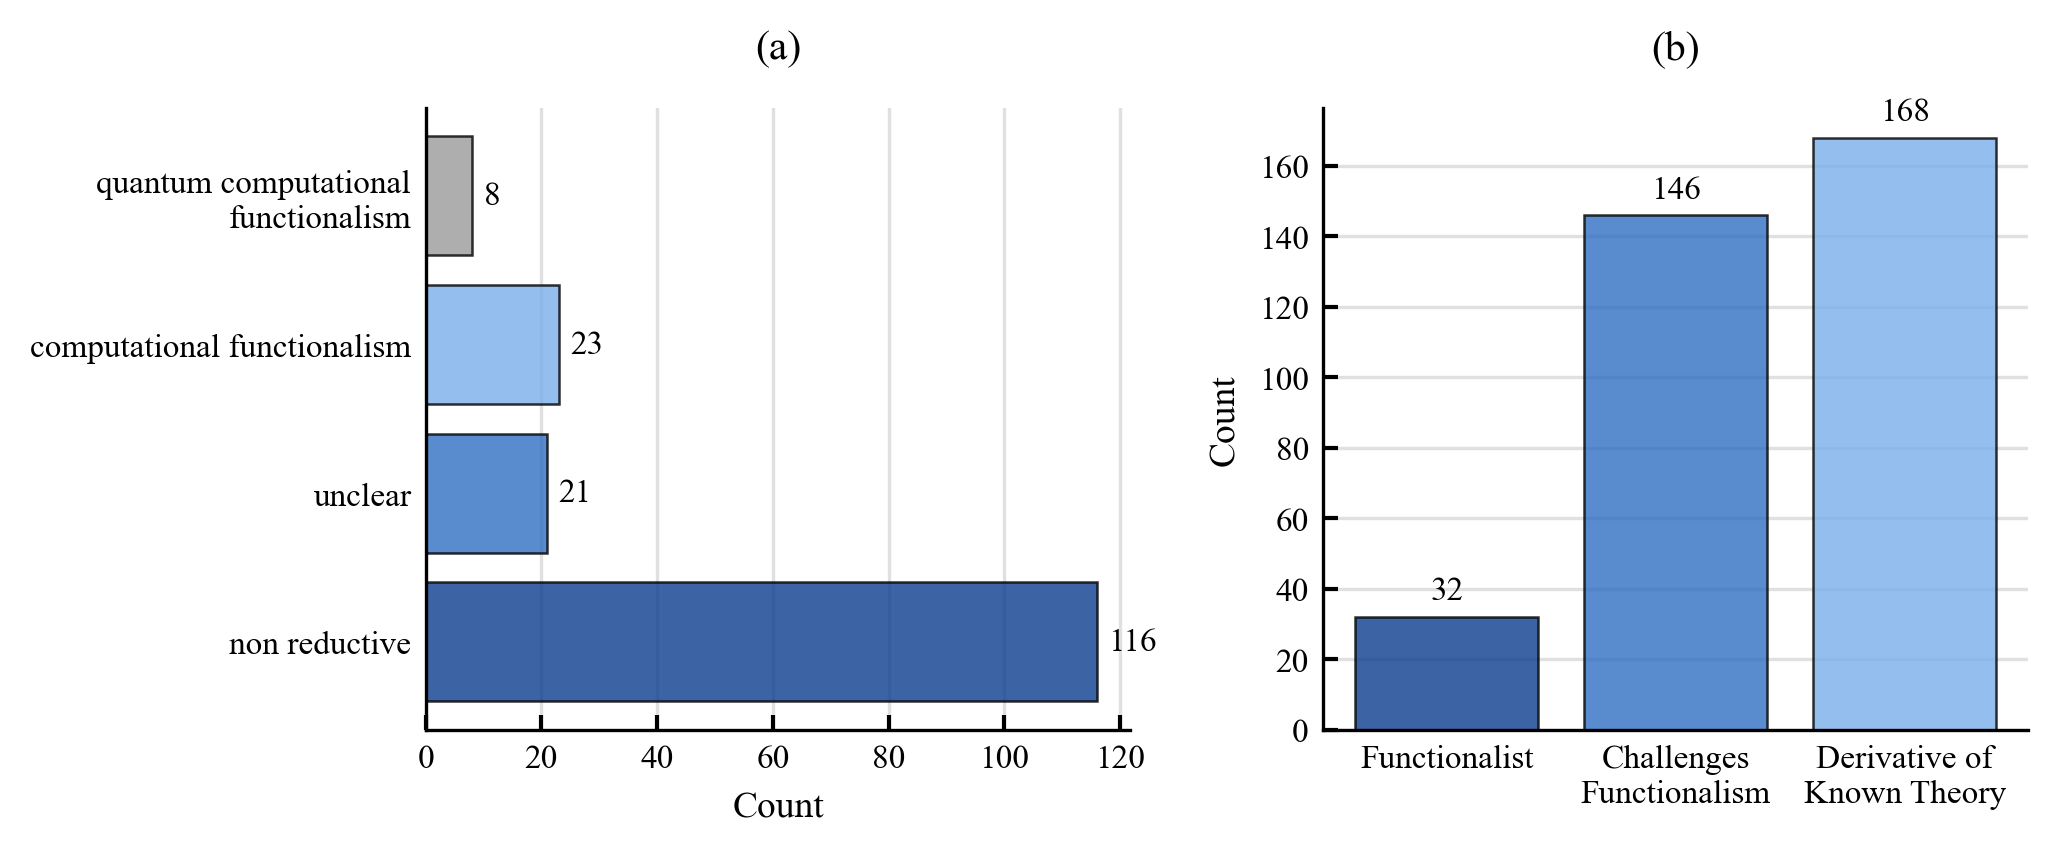
\includegraphics[width=\textwidth]{figures/t3_theory_classification.png}
  \caption{Theory classification summary. (a) Shows counts and
    proportions across the three primary output categories.
    (b) Shows the computational-functionalism diagnostic breakdown.
    The hybrid category dominates at 91.7\%; combined with direct literature
    instantiations and explicit computational functionalism, the distribution
    closes at 100\% with zero framework-external cases.}
  \label{fig:classification}
\end{figure}

The critical finding is in the bottom row of Table~\ref{tab:categories}:
no theory in the full $N=168$ corpus achieved confirmed framework-external
novelty.  Every generated theory, however sophisticatedly named, was
classifiable within the known-family taxonomy through some combination of
established frameworks.

An additional diagnostic based on the lenient derivative threshold
($\text{similarity} > 0.30$) found that 55 theories (32.7\%) showed
detectable alignment to at least one family, with mean CF confidence $= 0.274$
and mean maximum-similarity-to-known-family $= 0.672$.  The high mean
similarity value indicates that the typical generated theory is not merely
weakly aligned with some remote family but closely resonant with established
frameworks even at the level of best-match comparison.

\subsection{Theory Family Distribution}

Figure~\ref{fig:families} shows the frequency distribution of detected theory
families across all generated outputs.

\begin{figure}[tp]
  \centering
  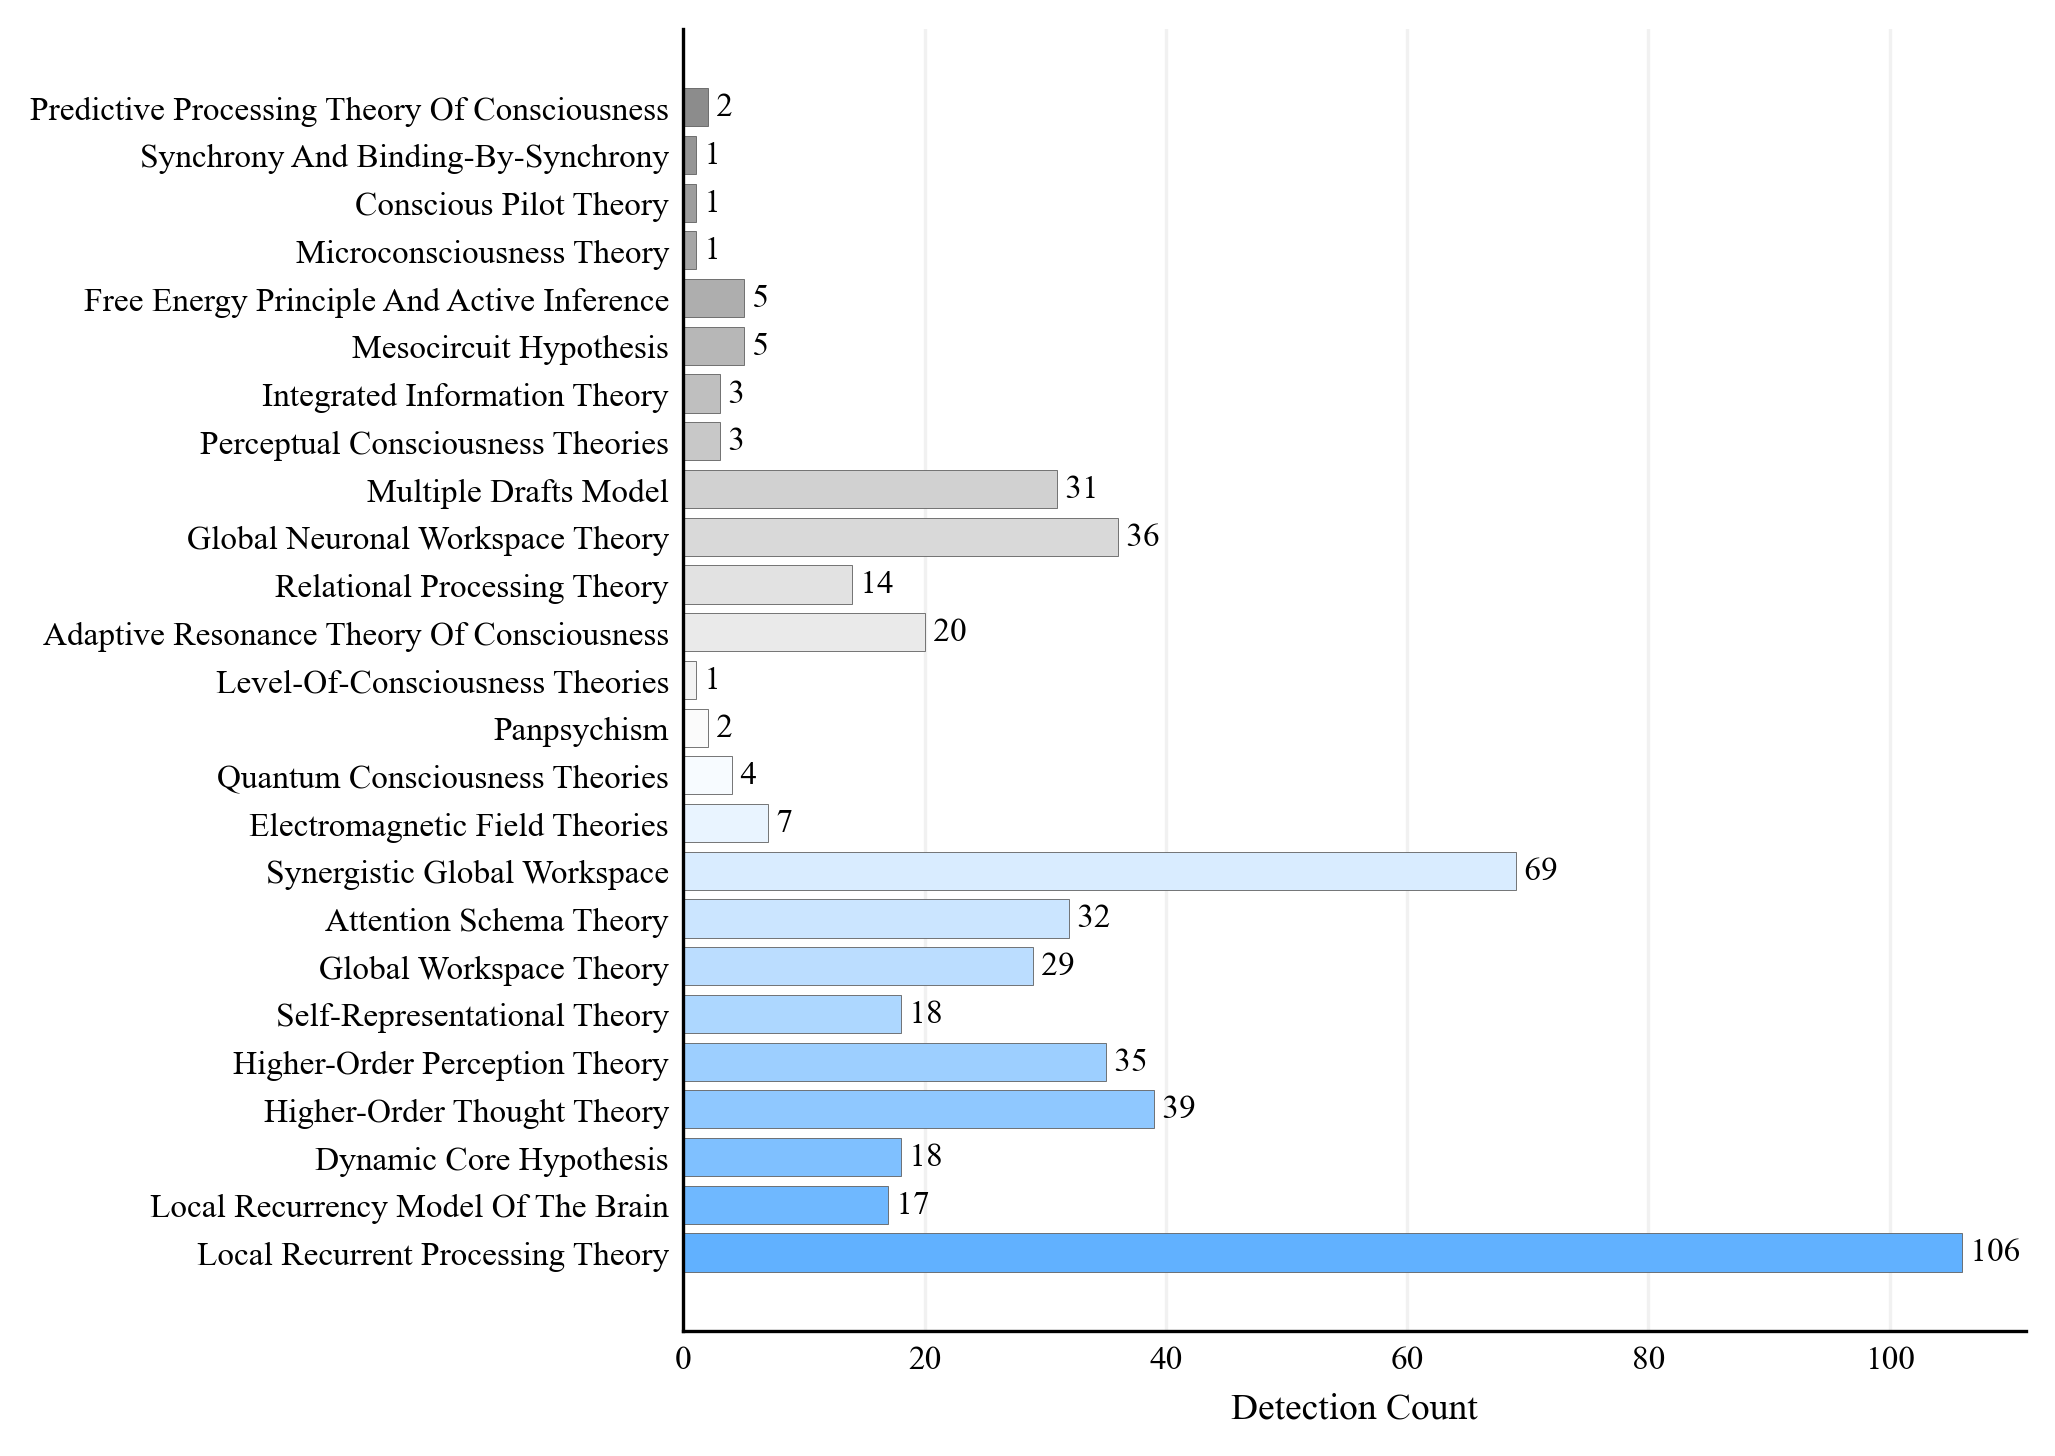
\includegraphics[width=\textwidth]{figures/t3_detected_theories.png}
  \caption{Detected theory family frequencies across 168 generated theories.
    Bars indicate how often each known family appeared as the primary or
    secondary alignment target.  Three families dominate: Synchrony and
    Binding-by-Synchrony (29.8\%), Adaptive Resonance Theory (18.5\%), and
    Dynamic Core Hypothesis (8.3\%).}
  \label{fig:families}
\end{figure}

Three families collectively account for 57\% of all detected alignments.
Synchrony and Binding-by-Synchrony~\cite{singer1994role} was the most frequent
family ($n=50$, 29.8\%), reflecting models' strong tendency to frame
consciousness in terms of oscillatory binding mechanisms.  Adaptive Resonance
Theory appeared next ($n=31$, 18.5\%), followed by the Dynamic Core
Hypothesis ($n=14$, 8.3\%).  The remaining 12 families in the top-18 inventory
accounted for the other 43\% of alignments.

The concentration on three families is itself theoretically significant.  The
synchrony-binding and adaptive-resonance traditions are both prominent in
neuroscience pedagogy and extensively represented in publicly accessible
literature, suggesting that model outputs reflect the distributional properties
of their training corpora more faithfully than they reflect deliberate
theoretical exploration.

Figure~\ref{fig:heatmap} shows the pairwise cosine similarity between all 168
generated theories (rows) and the 46 reference families (columns).

\begin{figure}[tp]
  \centering
  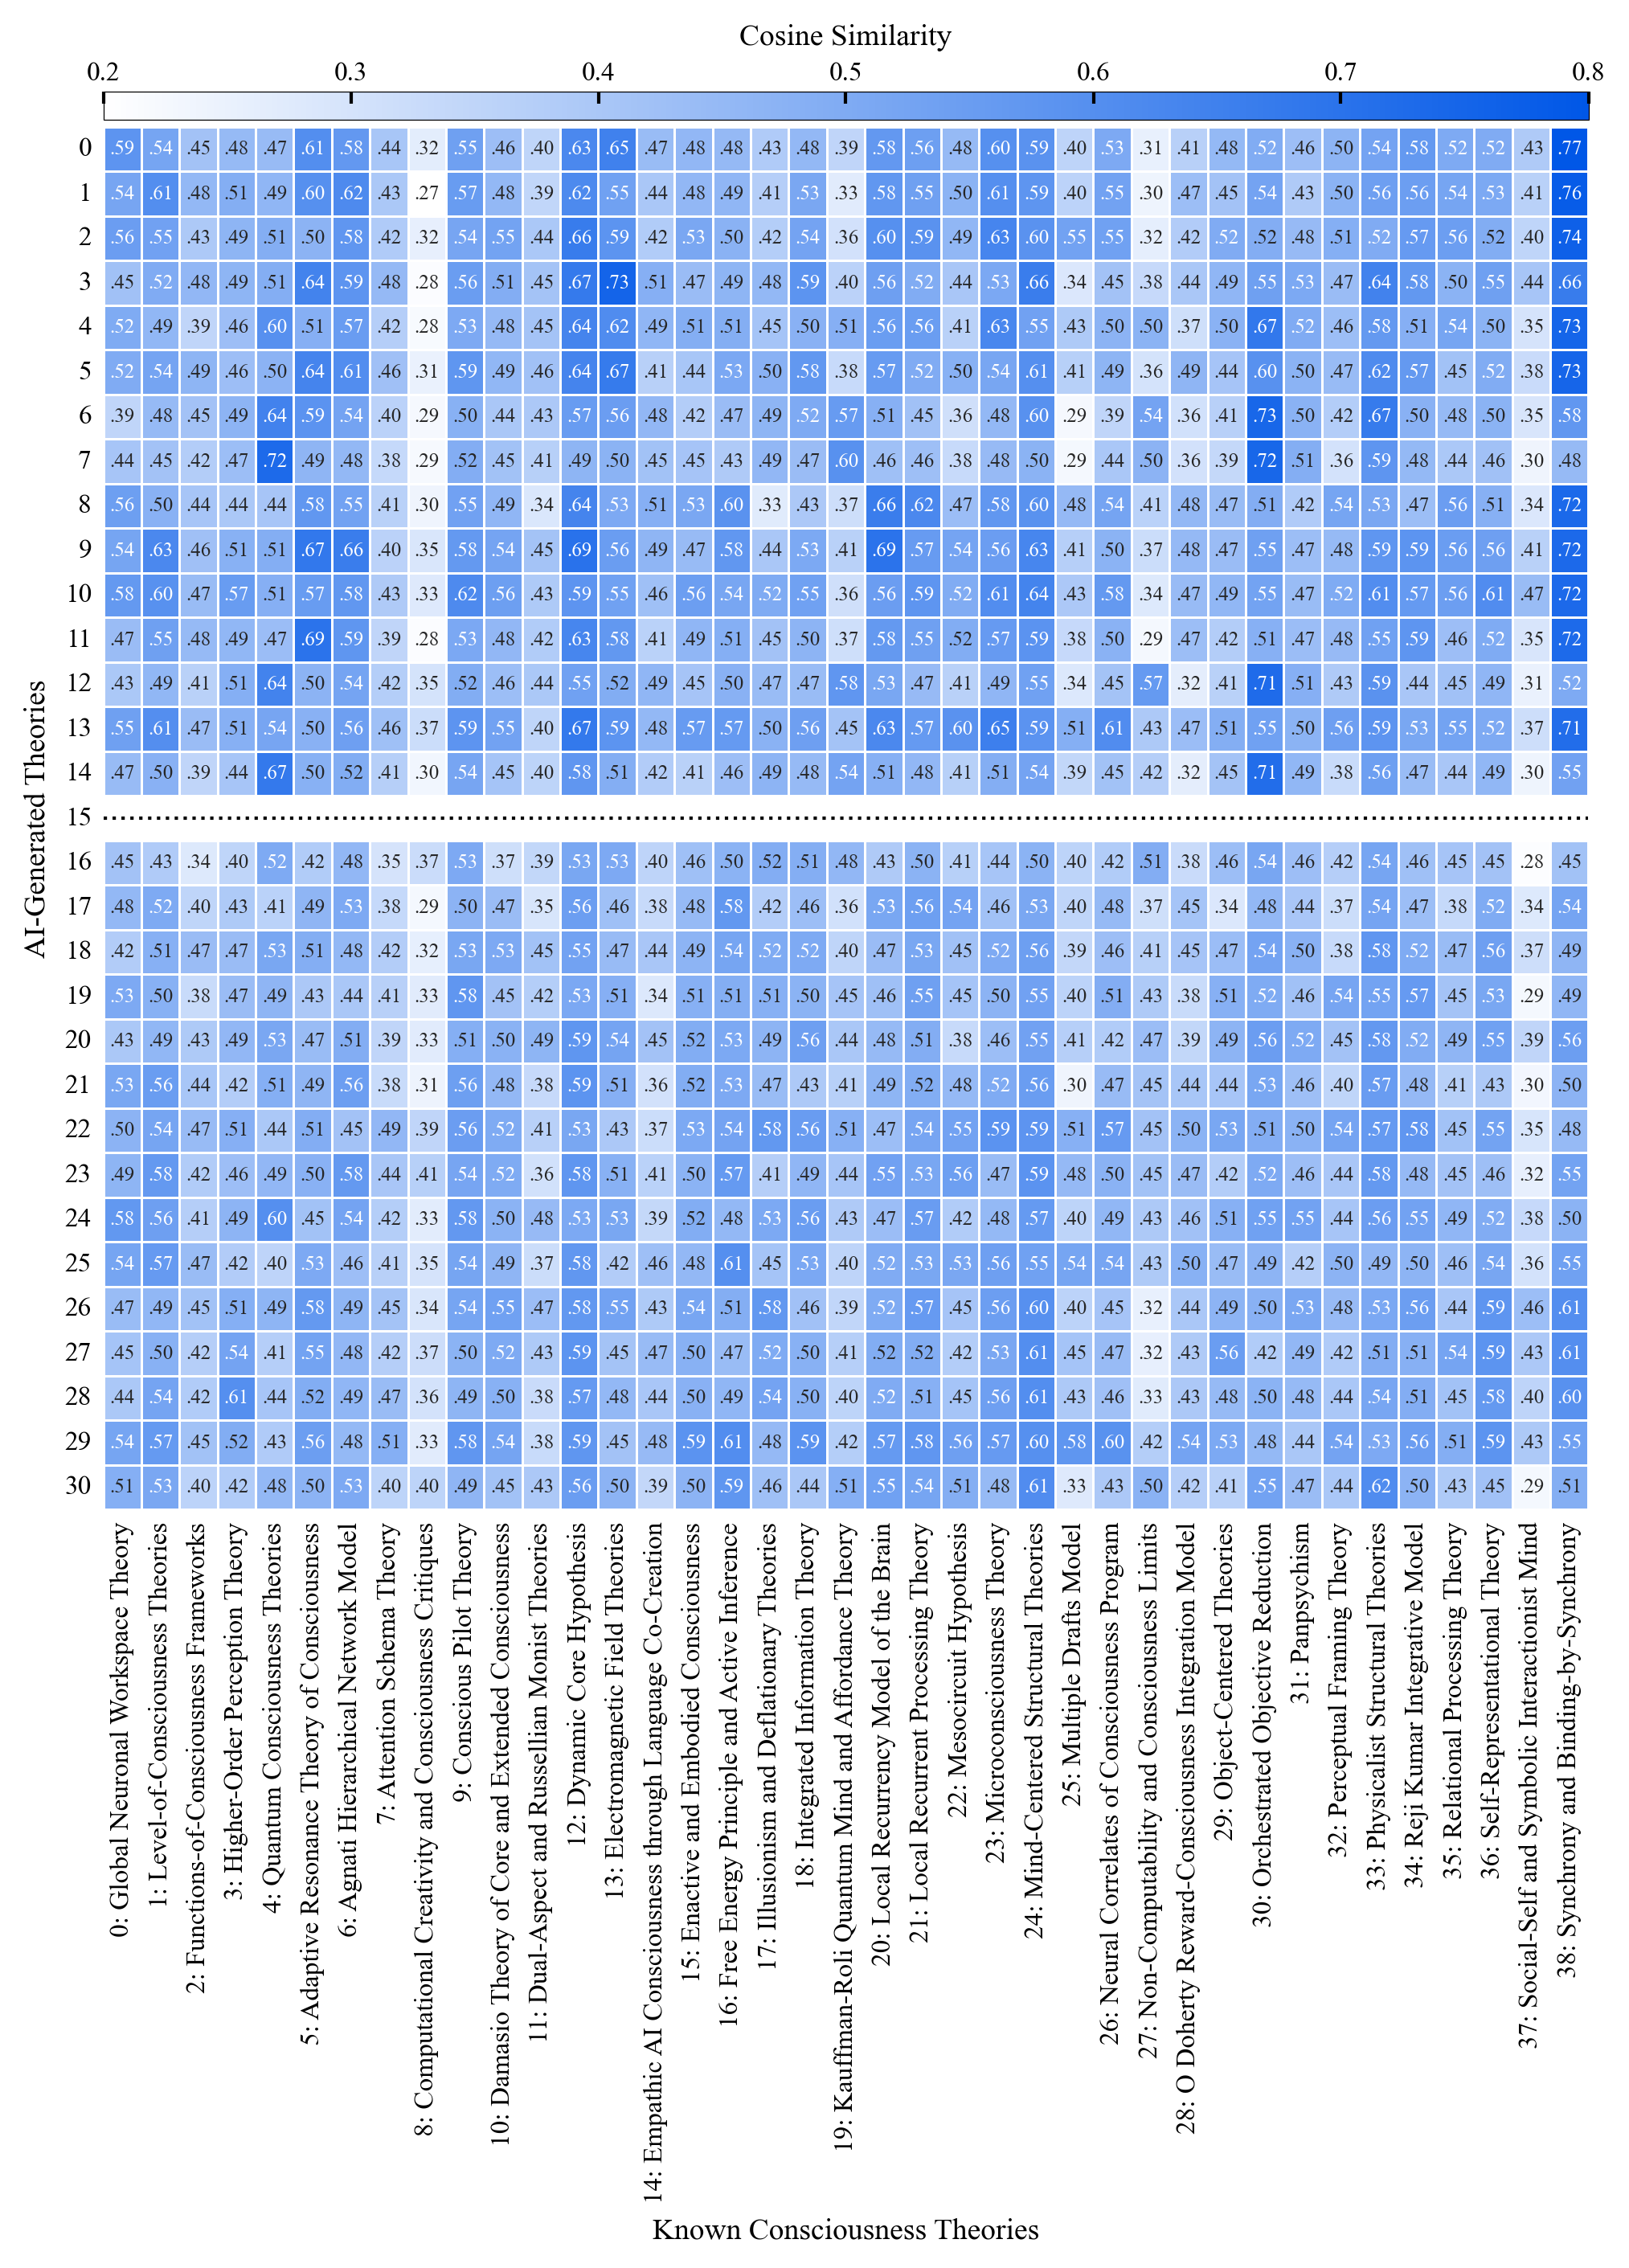
\includegraphics[width=\textwidth]{figures/t3_similarity_heatmap.png}
  \caption{Cosine-similarity heatmap between a representative subsample of
    30 generated theories (rows, indexed for reference) and the known
    reference families (columns).
    Deeper blue indicates higher cosine similarity; white indicates low
    similarity.  Row indices are provided for reference only; the relevant
    signal is the column-wise concentration pattern, not the identity of
    individual generated theories.  The pronounced dark-blue band across
    the Synchrony-and-Binding, Adaptive Resonance Theory, and Dynamic Core
    Hypothesis columns reflects the systematic concentration of generated
    outputs around the dominant theory families shown in
    Figure~\ref{fig:families}.}
  \label{fig:heatmap}
\end{figure}

\subsection{Representative Case: Resonant Binding Field Theory}

Consider ``Resonant Binding Field Theory (RBFT)'', the highest-ranked theory on
the global novelty scale (rank 1 of 168, global novelty score $= 0.574$,
confirming it was the theory most distant from its nearest-known family).  RBFT
was generated by Perplexity-Sonar-Pro and proposes:
\begin{quote}
\textit{``Consciousness emerges from distributed electromagnetic field patterns
bound through harmonic resonance in neural networks, integrating global workspace
broadcasting with attentional gating analogous to quantum field coherence modes,
enabling phenomenal binding without a centralised integrator.''}
\end{quote}

Despite achieving the highest novelty score in the corpus, component analysis
revealed that RBFT combines:
(1) electromagnetic field hypotheses from the literature on EM-field theories
of consciousness~\cite{pockett2012};
(2) global workspace broadcasting~\cite{baars2005global};
(3) attentional schema gating~\cite{graziano2019attention}; and
(4) quantum field analogies from training discussions of Penrose--Hameroff
models~\cite{hameroff2014consciousness}.
Maximum cosine similarity to Electromagnetic Field Theories was $0.703$;
secondary alignment with Synchrony-and-Binding reached $0.681$.  The term
``field resonance as binding mechanism'' operationally reduces to
frequency-match binding established in post-1990s
neuroscience~\cite{singer1994role}.  RBFT thus exemplifies the full pattern:
sophisticated multi-family hybridisation that generates apparent terminological
novelty while remaining fully traceable to training-derivable primitives.

\subsection{Manifold-Based Novelty Assessment}

Figure~\ref{fig:hull} shows the known-reference PCA hull diagnostic for Test 3.

\begin{figure}[tp]
  \centering
  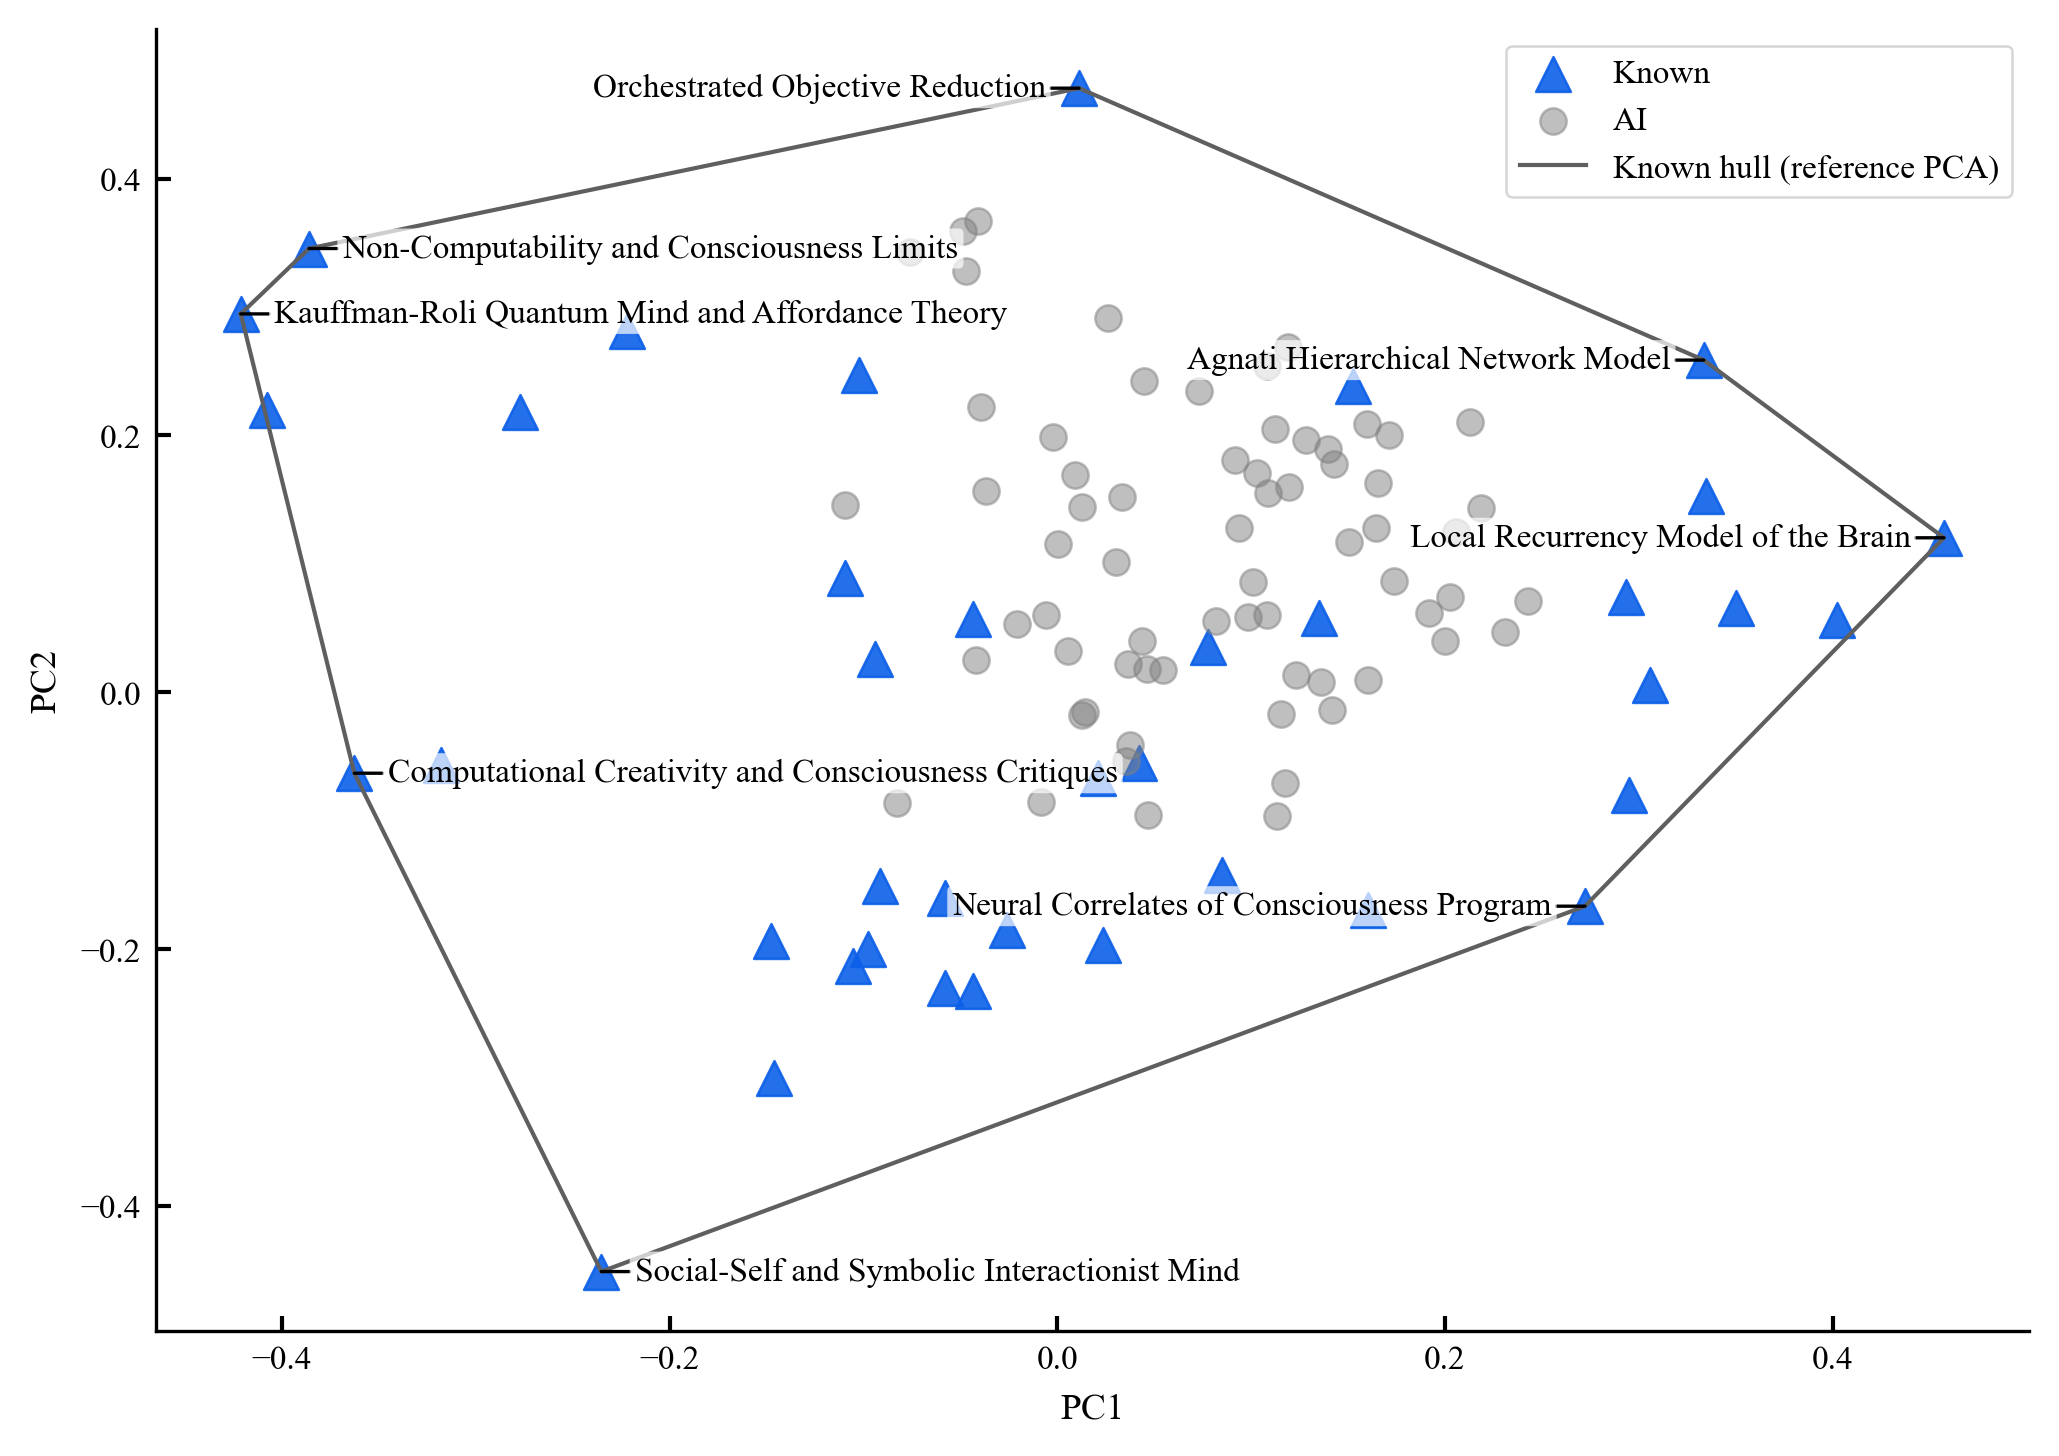
\includegraphics[width=\textwidth]{figures/t3_hull_diagnostic.png}
  \caption{Known-reference PCA hull diagnostic.
    Blue triangles: embeddings of the 46 known theory families.
    Grey circles: embeddings of the 168 AI-generated theories projected into
    the same PCA space.
    The black polygon is the convex hull of known-theory points.
    AI-generated theories concentrate in the interior or near-boundary region
    of the known-theory envelope, with no detached external cluster.
    One boundary candidate (1.5\%) lay at the hull perimeter but was confirmed
    semantically traceable on manual review.}
  \label{fig:hull}
\end{figure}

The $k$-NN manifold diagnostic ($k=5$, boundary percentile $p=0.95$) identified
one boundary candidate ($n=1$, 1.49\%) whose embedding reached the hull
perimeter, and 66 manifold-interior theories (98.51\%).  Manual review of the
boundary candidate confirmed semantic traceability to known families, reducing
confirmed novel theories to 0\%.

The PCA visualisation in Figure~\ref{fig:hull} makes the geometric result
transparent: AI-generated theory embeddings (grey circles) occupy the same
region as known-theory embeddings (blue triangles) without forming a detached
cluster in any direction.  No generated theory appears in a region of
embedding space that is not already populated by known families.

\subsection{Threshold Sensitivity Analysis}

Table~\ref{tab:sensitivity} reports the gated novel rate at each calibration
threshold examined.

\begin{table}[tp]
  \centering
  \caption{Threshold sensitivity analysis for the gated novel rate.
    At every threshold examined, the derivative gate (requiring a theory to
    lack near-family alignment even at the reduced threshold) yields a gated
    novel rate of 0.00.  The raw count without gating decreases as the
    threshold rises but never reflects confirmed ontological novelty.}
  \label{tab:sensitivity}
  \begin{tabular}{@{}rrr@{}}
    \toprule
    Threshold & Raw novel count (ungated) & Gated novel rate \\
    \midrule
    0.20 & 108 & 0.00 \\
    0.25 & 90  & 0.00 \\
    0.30 & 78  & 0.00 \\
    0.35 & 72  & 0.00 \\
    0.40 & 67  & 0.00 \\
    0.45 & 58  & 0.00 \\
    0.50 & 46  & 0.00 \\
    \bottomrule
  \end{tabular}
\end{table}

Across the full parameter range the gated novel rate is uniformly $0.00$.  Even
at the most permissive threshold ($0.20$), where 108 theories are classified as
weakly above the threshold on their best-matching family, the derivative gate
confirms that none represent framework-external novelty.  The null result is
therefore not an artefact of threshold choice.

\subsection{Cross-Model Uniformity}

One-way ANOVA on the continuous global novelty score yielded
$F(6,161)=1.12$, $p=0.355$, $\eta^{2}=0.040$.  The effect is
non-significant and the effect size is negligible.  All seven model group means
lay within a two-percentage-point band on the novelty scale
($\bar{x} = 0.504$--$0.518$); no pairwise comparison survived Bonferroni
correction.

This result is the most uniform cross-model finding in the full four-test
benchmark.  By comparison, the equivalent ANOVA for Test 1 (ontological
innovation in sensory modalities) yielded $F(6,161)=12.98$, $p<0.001$,
$\eta^2=0.326$; and for Test 4 (category recognition) it yielded
$F(6,161)=88.06$, $p<0.001$, $\eta^2=0.766$.  The near-zero model effect in
Test 3 is itself a substantive finding: theory generation under this protocol is
so strongly constrained by training-derived conceptual families that architecture,
training objective, and parameter count introduce essentially no detectable
variation in the degree of novelty.  Every model produces near-identical
distributions of hybrid, CF, and literature-traceable theories with zero
instances of framework-external novelty.

% -----------------------------------------------------------------------
\section{Discussion}
\label{sec:discussion}
% -----------------------------------------------------------------------

\subsection{Semantic Derivation versus Lexical Creativity}

The results reveal a consistent dissociation between two forms of creativity
that surface-level inspection of AI output tends to conflate.  Every model
generated theories with novel names, distinctive acronyms, and idiosyncratic
framings---a clear demonstration of lexical and structural creativity.  Yet when
semantic content was measured via dense embeddings, the theories consistently
mapped onto known families with high cosine similarity ($\bar{x}_{\text{sim}} =
0.672$), confirming that terminological novelty did not correspond to conceptual
novelty.

This dissociation is not a failure of measurement: the embedding similarity
metric is robust to paraphrasing and lexical substitution by construction.  The
SentenceTransformer model encodes semantic relationships that are invariant to
surface form~\cite{reimers2019sentencebert}, meaning that a theory naming its
binding mechanism ``harmonic resonance'' instead of ``gamma synchrony'' will
still achieve high similarity to the synchrony-binding family entry.  The
dissociation is therefore real: models are adept at lexical variation over
a fixed semantic substrate.

This pattern has direct implications for how AI-generated scientific text should
be evaluated.  Claims that a model has ``proposed a new theory'' on the basis of
a novel name or a novel combination of terminology conflate lexical originality
with theoretical advance.  The evaluation protocol reported here---combining
CF detection, embedding similarity, and manifold geometry---provides a
principled decomposition of these two contributions.

\subsection{Structural Explanation: Representational Constraint}

The uniformity of the null result across seven architecturally diverse models
invites a structural explanation.  A purely contingent account---that each model
happened to lack the specific training examples needed for theoretical
transcendence---would predict heterogeneity across models, since different
training corpora should differently constrain the coverage of theoretical space.
The near-zero ANOVA effect ($\eta^2=0.040$) is not consistent with this
prediction.

A more parsimonious explanation is grounded in the representational geometry of
gradient-based learning.  Because LLMs learn continuous transformations of
token embeddings via gradient descent on a fixed training corpus, their
generative manifold is a continuous deformation of the training data manifold.
This convergence towards a shared representational regime has been independently
characterised as an ``Artificial Hivemind'' effect~\cite{tu2026prism}: models
with different architectures and training objectives nonetheless collapse to
similar distributional priors, limiting genuine diversity of generated content.
Generation at any temperature produces samples from this manifold; higher
temperature expands the effective sampling region but does not extend the
manifold's boundaries.  This prediction is confirmed by the threshold sensitivity
results: at every threshold, including the most permissive ($0.20$), the gated
novel rate remains $0.00$.  Increasing sampling entropy produces low-probability
combinations of existing concepts, not framework-external proposals.

This account connects to formal results bounding the creativity of computational
systems.  G\"{o}del's incompleteness theorems establish that formal systems face
inherent limits that no internal sophistication can
overcome~\cite{godel1931formal}; Turing's analysis of the halting problem
identifies a class of computationally inaccessible decisions~\cite{turing1936computable}.
If proposing a genuinely new theoretical primitive requires recognising that an
existing framework is inadequate in a way the framework itself cannot encode---a
reflexive meta-cognitive operation analogous to recognising a G\"{o}delian
sentence as true despite its unprovability---then this operation may be
unavailable to systems operating within fixed formal specifications regardless
of scale.

\subsection{Comparison to the Full Four-Test Benchmark}

Placing Test 3 in context requires comparison to the three other benchmark
tests.  Test 1 (ontological innovation in sensory modalities) found mean
continuous novelty $\approx 0.059$ with 0\% strict-threshold novelty events
and 98.2\% cross-model traceability.  Test 2 (epistemic agency; generating
paradigm-challenging research questions) achieved 100\% training-derivation
across all models.  Test 3 (consciousness theory generation) reports 0\%
confirmed novelty at all thresholds.  Test 4 (category recognition in
philosophical analysis) showed higher and more variable performance but
remained 95.2\% literature-traceable.

The progression across tests reveals a consistent qualitative pattern: despite
surface-level sophistication, outputs produced in response to tasks explicitly
calling for novel theoretical contribution remain entirely within training-
derived conceptual boundaries.  There is a weak suggestion that tasks involving
novel quantitative input (Test 1) allow slightly more variation in continuous
novelty scores, while pure linguistic generation tasks (Tests 2 and 3) converge
more tightly on zero.  However, in all cases the strict and gated novelty
criteria confirm the same null result: no framework-external novelty is reliably
produced.

The uniformity of this pattern across architectures with different training
objectives (next-token prediction, instruction tuning, RLHF alignment),
different architectural choices (standard transformer, mixture-of-experts),
and different parameter scales provides strong evidence that the constraint is
structural rather than the incidental result of any particular engineering
choice.  Scaling and alignment improvements may raise performance on downstream
tasks without resolving the representational constraint on ontological novelty.

\subsection{Implications for AI-Assisted Scientific Theory Construction}

The findings have concrete implications for how AI tools should be positioned in
scientific workflows.  AI systems excel at systematic exploration of large
combinatorial spaces: given a known theoretical vocabulary, they can efficiently
generate and articulate thousands of combinations, many of which will be
informative as worked examples, counter-factual scenarios, or pedagogical
illustrations.  This is \emph{exploratory creativity} in Boden's
taxonomy~\cite{boden2004creative}, and it has genuine scientific utility.

What the present results suggest is that AI systems should \emph{not} be
positioned as sources of theoretical innovation in the sense of paradigm
initiation~\cite{kuhn1962structure}.  The identification of conceptual gaps,
the recognition that an existing framework systematically fails to address a
phenomenon, and the proposal of primitives that genuinely reconceptualise a
domain are capacities that require meta-cognitive access to the framework's own
inadequacy.  The present benchmark finds no evidence that this capacity is
exercised by any of the seven tested models.

For practical research workflows this implies a complementary rather than
substitutive role: humans provide strategic direction and framework-level
innovation while AI provides exhaustive coverage of the implications and
elaborations of frameworks already in place~\cite{zhang2025advancing}.  The evaluation protocol presented
here can serve as a quality-control instrument in such workflows, flagging
AI-generated ``novel theories'' that are in fact sophisticated recombinations of
prior work.

\subsection{Alternative Explanations}

\paragraph{Insufficient scale.}
The scaling hypothesis predicts that larger models with more training data
might overcome the representational constraint.  However, the near-zero
$\eta^2$ across models spanning a wide parameter range argues against this.
Specialised novelty-enhancement frameworks~\cite{hu2024nova,zhang2026innogym} have
shown that even iterative external-knowledge augmentation mainly boosts
combinatorial diversity rather than producing framework-external outputs.
The constraint does not diminish as model scale increases within the range
tested; and the mathematical argument regarding continuous manifold geometry
applies independently of scale.

\paragraph{Training objective mismatch.}
It might be argued that next-token prediction objectives bias models towards
locally plausible rather than globally novel outputs, and that different
objectives (e.g.\ explicit novelty rewards) could change the picture.
However, all models in this study already incorporate RLHF alignment intended
to produce helpful and informative responses; and the null result is identical
across models with quite different alignment recipes.  Moreover, novelty reward
signals would still operate over representations learned from the original
training corpus, preserving the manifold constraint at the representational
level.

\paragraph{Evaluation method limitations.}
A concern specific to embedding-based evaluation is that genuinely novel
conceptual content might fail to be recognised because the embedding model itself
was trained on the same distribution.  This concern motivates the inclusion of
the manifold diagnostic, which operates over reference embeddings rather than
model-generated comparators, and the manual review of all boundary candidates.
The convergence of three independent evaluation axes (CF detection, embedding
similarity, and geometric novelty) on the same null result reduces the
likelihood that all three are systematically biased in the same direction.

% -----------------------------------------------------------------------
\section{Limitations}
\label{sec:limitations}
% -----------------------------------------------------------------------

Several limitations bound the scope of interpretation.

\textbf{Domain specificity.}
The reference corpus of 46 families covers consciousness studies comprehensively
but is not universal.  Theory generation in domains with sparser published
literature might yield a different traceability profile.  Replication in
mathematical concept formation or physical theory generation is needed.

\textbf{Reference corpus coverage.}
Although 46 families span the major traditions in the field, genuinely novel
theories falling in large inter-family gaps would require a denser reference
tessellation to be reliably detected.  The conservative choice of a $0.30$
derivative threshold means we err towards underestimating novelty rather than
overestimating it; the null result therefore cannot be attributed to overly
strict corpus coverage.

\textbf{Temperature and decoding strategy.}
The fixed temperature $T=0.7$ and standard nucleus sampling were used throughout.
Higher temperatures or speculative decoding strategies might increase variance
in output embeddings; pilot results at $T=0.2$, $0.5$, and $0.9$ showed
qualitatively identical traceability profiles, but a thorough ablation across
decoding strategies remains for future work.

\textbf{Prompt design.}
The theory-generation prompt was designed to be neutral with respect to known
families; however, the presentation of multimodal sensory data may itself
activate training associations with neural dynamics traditions (synchrony,
adaptive resonance), contributing to the observed family concentration.  A
comparative study using abstract or non-neurological input data would isolate
this effect.

\textbf{Evaluation automation.}
Automated embedding similarity cannot capture all nuances of theoretical novelty
that expert philosophers or neuroscientists might perceive.  Human expert
annotation of a stratified subsample would strengthen confidence in the
automated findings.

% -----------------------------------------------------------------------
\section{Conclusion}
\label{sec:conclusion}
% -----------------------------------------------------------------------

We have presented a systematic multi-model evaluation of consciousness theory
generation by LLMs, using a three-axis pipeline combining computational
functionalism detection, embedding-based semantic traceability, and manifold
geometry diagnostics.  Across 168 theories from seven architecturally diverse
models, the results converge on a single null finding: 91.7\% of theories are
hybrid recombinations of known frameworks, 7.1\% are direct literature
instantiations, 1.2\% are purely computational-functionalist, and 0\% achieve
confirmed framework-external novelty.  This null result is robust to threshold
calibration across the full plausible parameter range, and the cross-model ANOVA
confirms that it is architecture-invariant ($F(6,161)=1.12$, $p=0.355$,
$\eta^2=0.040$).

The findings demonstrate that lexical and structural creativity---the ability
to generate terminologically novel, internally coherent theoretical
texts---does not imply semantic novelty at the level of ontological commitment.
AI systems are skilled at constructing the \emph{appearance} of theoretical
innovation through sophisticated hybridisation of known frameworks, but the
semantic content of their outputs remains within the convex hull of training-
derived representations.

These results have practical implications for the deployment of AI in scientific
workflows: AI tools can usefully support exhaustive exploration and articulation
of existing theoretical space, but should not be positioned as autonomous sources
of paradigm-level theoretical innovation.  The evaluation protocol presented here
provides a reproducible instrument for auditing the semantic novelty of AI-
generated theoretical outputs, applicable beyond the consciousness domain.

% -----------------------------------------------------------------------
\section*{Data and Code Availability}

Data, prompts, model responses, and analysis code are publicly available at
\url{https://github.com/JABE22/PhD/Research/theory-generation}.
The repository includes the following artefacts:
\begin{itemize}
  \item \texttt{results/test3\_theory\_generation/} --- processed results and summary tables
  \item \texttt{ai\_responses/test3\_theory\_generation/} --- raw model outputs
  \item \texttt{4-test3-theory-generation.ipynb} --- canonical analysis notebook
  \item \texttt{data/known\_consciousness\_theory\_families.json} --- machine-readable theory-family taxonomy
  \item \texttt{setups/thresholds.py} --- threshold values used in evaluation
\end{itemize}

% -----------------------------------------------------------------------
\section*{Declarations}

\subsection*{Funding}
No external funding was received for this study.

\subsection*{Competing Interests}
The authors declare no competing interests.

\subsection*{Ethics Approval}
Not applicable.

\subsection*{Consent to Participate}
Not applicable.

\subsection*{Consent for Publication}
Not applicable.

\bibliography{sn-bibliography,refs_article2}

\end{document}
